\chapter{Theory}

\section{On Standard Model of Particle Physics}

\textbf{Forward}

It is the goal of this section to succinctly (in a relative sense) derive the 
principal aspects of the  standard model of particle physics from fundamental principles. 
The questions to be answered answered are: how do we build a complex framework consisting of 
a variety of particles and interactions that  experimentally describes the univerise (neglecting
 gravity) with startling accuracy? what are the guiding principles? and despite its success, why
is the theory incomplete?

First we will describe the lagrangian formulation of classical mechanics. From here we introduce, 
classical field theory and the fundmantal quantization of quantum mechanics to arrive at quantum field
theory (QFT). After a brief discussion of global and local lagrangian symmetries in a QFT, we discuss
gauge theories and how local gauge symmetries give rise to the interactions mediating the 
fundamental forces excluding gravity. Ultimately, we review spontaneous 
electroweak symmetry breaking as the source of the gauge boson masses and the higgs field. 

\begin{itemize}
\item Energy and The Principle of Minimal Action: Here we will build up the concept
\item Symmetry and Local Gauge Symmetry: What symmetries do we enforce upon the form of our theory
and what are the consequences.
\item Theory Renormalizability: What limits the type of terms we can include in our lagrangian as to preserve
the ability to calculate the outcomes of simple scattering processes. 
\end{itemize}

\subsection{Getting to Quantum Field Theory}

\subsubsection{Lagrangian Mechanics}

In lagrangian mechanics, the time evolution of some generalized coordinate $q$ can
 be determined via the principle of minimal action $\delta S = 0$. 
\begin{align*}
S[q(t)] &= \int_{t_1}^{t_2} L \left(q,\frac{dq}{dt},t\right) dt
\end{align*}
where $S$ is a functional of the time dependent generalized coordinate $q(t)$. 
Let $\dot{q} = \frac{dq}{dt}$ The equations of motion are derived by varying S
\begin{align*}
\delta S &= \int_{t_0}^{t_1} \left [ \frac{\partial L}{\partial \dot q}  \delta \dot q + \frac{\partial L}{\partial q} \delta q \right ]dt 
\end{align*}
Note that $\delta \dot q = \delta\frac{dq}{dt} = \frac{d(\delta q)}{dt}$. 
Integrate the first term by parts, and require that $\delta q$ vanish at the boundaries:
\begin{align*}
\int_{t_0}^{t_1} \left [-\frac{d}{dt}\left (\frac{\partial L}{\partial \dot q} \right) \delta q + \frac{\partial L}{\partial q} \delta q \right ] dt  = \delta S = 0
\end{align*}
by the principle of minimal action we have arrived at the euler equations of motion:
\begin{align*}
\frac{d}{dt}\left (\frac{\partial L}{\partial \dot q} \right) = \frac{\partial L}{\partial q}  
\end{align*}
For a generic lagrangian with potential energy term $V(q)$, $L=\frac{1}{2}m_q \dot q^{2} - V(q)$  we obtain the equation of motion (or force law) $F=m\ddot{q}=-\frac{dV}{dq}$ 
\subsubsection{Classical Field Theory}
In comparison with classical mechanics, which deals with finitely many [cite:tong] general
 coordinates $q_i$, classical field theory deals with an infinite number of degrees of freedom 
$\phi_i(\vec x, t)$ [cite:tong] with a degree of freedom for each spatial coordinate  $\vec x,t$ and 
and index $i$. For simplicity we use a single index $\mu$ for the four spacetime dimensions and utilize
the einstein summation convetion where repeated indicies are summed over. 
The corresponding action can be written in terms of a lagrangian density $\mathcal{L}(\phi,\partial_\mu \phi)$
\begin{align*}
S = \int dt L = \int d^3x \int dt \mathcal{L}(\phi,\partial_\mu \phi) = \int dx^4 \mathcal{L}(\phi,\partial_\mu \phi)
\end{align*}
Similarlly, we arrive at classical Euler-Lagrange Equations of motion:
\begin{align*}
\partial_\mu \left( \frac{\partial\mathcal{L}}{\partial (\partial_\mu \phi)}\right) = \frac{\partial \mathcal{L}}{\partial\phi}
\end{align*}
We now consider the simple free lagrangian density for a real scalar field $\phi$:
\begin{align*}
\mathcal{L} = \frac{1}{2}\partial_\mu \phi \partial^\mu \phi - \frac{1}{2} m\phi^2 
\end{align*}
we have achieved a relativistically invariance for free as all indicies are contracted. To see this, consider a lorrentz transformation $\Lambda$ on the kinetic term. The transformation induces $\phi(x) \rightarrow \phi'(x) = \phi(\Lambda^{-1} x) = \phi (y)$. The transformation is $\Lambda$ as we actively
rotate the coordinate system rather than rotating the field. 
\begin{align*} 
\partial_\mu \phi \partial^\mu \phi \rightarrow& ((\Lambda^{-1})^\mu_\rho \partial^\rho \phi)( (\Lambda^{-1})_\mu^\nu \partial_\nu \phi) 
= \eta^{\rho\nu} \partial_\rho \phi \partial_\nu \phi 
= \partial^\nu \phi \partial_\nu \phi 
\end{align*}
where we have used the fact that the the spacetime metric is invariant under lorentz transformations.
\begin{align*}
\Lambda^\mu_\rho \eta^{\rho \lambda} \Lambda_{\lambda}^\nu = \eta^{\mu\nu}
\end{align*}
As the action integrates over all space time, the change of variable from $x\rightarrow y$ is
inconsequential and yield the same equations of  motion.
Applying the euler lagrange equation we arrive at the 
classical relativistcally invariant klein gordon equation:
\begin{align*}
(\partial^2 - m^2 ) \phi = 0
\end{align*}
taking the fourier transform of state $\phi$:
\begin{align*}
\phi(\vec x, t) = \int \frac{d^3p}{(2\pi)^3} e^{-i \vec p \cdot \vec x } \phi (\vec p, t)
\end{align*}
Note that the $(2\pi)^3$ is a normalization convention on the field. We see that the solution satsifies:
\begin{align*}
\left( \frac{\partial^2 }{\partial t^2} + (p^2 + m^2) \right ) \phi(\vec p, t)= 0
\end{align*}
From this we recognize that this is just the equation of motion for
 a harmonic oscillator with energy $\omega^2 = p^2 + m^2$

\subsubsection{The Canonical Quantization}

Quantum mechanics consists of 4 fundamental postulates. Here we enumerate their classical counter parts [cite.schrednicki]

\begin{enumerate}
\item \textbf{Particle State}: In classical mechanics a the state of a particle is determined by two variables $x(t)$ and $p(t)$. In quantum mechanics, the state is a a vector $|\psi \rangle$ in a hilbert space $\mathcal{H}$
\item \textbf{Dynamic Variables }: Clasically, all dynamical variables are a
 function only $x(t)$ and $p(t)$. In quantum mechanics, classical variables 
represented as a function of $x$ and $p$ are instead 
represented by hermitian operators $X$ and $P$ that statisfy the commutation 
relation $[X,P] = \frac{i}\hbar$. 
\item \textbf{Measurement}: Clasically, the particle state is unaffected by measurement and strictly
deterministic based on the values of $x$ and $p$. Quantum mechanically, a particle in a state $|\psi \rangle$ when measured will yield and eigenvalue $\omega$ of the operator $\Omega$ with probability
$|\langle\omega|\psi \rangle|^2$. After measurement the particle state is the corresponding eigenvector  $|\omega\rangle$
\item \textbf{Time Evolution}: Classically, $p$ and $x$ change with time according to hamiltons (or lagrangian) equations of motion. Quantum mechanics asserts the state vector evolves with time according to the
Schrodinger equation: $i \hbar \frac{d}{dt}|\psi(t) \rangle = H | \psi(t) \rangle$. Where $H$ is the 
hamiltonian with classical $p$ and $q$ replaced by the corresponding quantum mechanical operators
\end{enumerate}

The canonical quantization consists of the second postulate that that measurement of postition
and momentum do not commute (postulate 2). This is the source of the famous heisenburg uncertainty
principle that there are no simultaneously measurable states of $p$ and $q$. 

If we consider the quantum harmonic oscillator with hamiltonian:
\begin{align*}
H = \frac{p^2}{2} + \frac{1}{2}\omega^2 q^2
\end{align*}
and postulate the existance of the creation ($a^\dagger$) and annihilation ($a$) operators:
\begin{align*}
a &= \sqrt{\frac{\omega}{2}}q + \frac{1}{\sqrt{2\omega}}p \text{  } a^\dagger &= \sqrt{\frac{\omega}{2}}q - \frac{1}{\sqrt{2\omega}}p 
\end{align*}
which corresponding give the 
\begin{align*}
q = \frac{1}{\sqrt{2\omega}} (a + a^\dagger) \text{  } p = -i \frac{\omega}{2}( a - a^\dagger) 
\end{align*}
 substituting into the hamiltonian we find a simple solution after applying
the commutation relation $[p,q]=-i$ (where we have set $\hbar=1$):
\begin{align*}
H =  \omega(a^\dagger a + \frac{1}{2}) 
\end{align*}
Importantly we see via the relation $[H,a]|E\rangle = (E-\omega)a|E\rangle$ and 
$[H,a^\dagger]|E\rangle = (E+\omega)a^\dagger|E\rangle$ that the operators raise and 
lower the harmonic oscillator in multiples of $\omega$. The energy levels are quantized 
in units of $\omega$. Also called ladder operators, $a$ and $a^\dagger$, raise and lower
the energy state by 1 unit of $\omega$ with a ground state energy $\frac{\omega}{2}$. 

If we now consider knowledge of classical field theory we can build a quantum field by
promoting the coordinate $q$ to a field $\phi$. We now write
the solution to the Klein-Gordon equation as an infinite sum of creation and 
annihilation operators that create or destroy a particle with energy $\omega_p^2 =
p^2 + m^2$ designated by its four-momentum $p$. Taking the solution to fourier space:
\begin{align*}
\phi = \int d^4x \frac{1}{\sqrt{2\omega_{p}}} \left [  a_p e^{ipx} + a_p^\dagger e^{-ipx} \right ]
\end{align*} 

Although result only applies for a real scalar field (spin 0), the corresponding feminoic field (spin 1/2)
field can be found similarlly starting from the dirac equation. 

\subsection{Symmetries}

\textbf{Noether's Theorem}

It cannot be understated the importance and the consequences of symmetries in the standard model. The
invariance of the action (equivalently the equations of motion) under linear translations of the  coordinates
gives rise to conservation of momentum. Simillarly,  rotations of the coordinate space
yields the conservation of angular momentum. This is a consequence of noether's theorem, that every 
continuous symmetry of the action has a corresponding conservation law. 

To be concrete, let us consider an action that is invariant under some field transformation
 $\phi \rightarrow \phi + \delta \phi$. If we consider a gauge transformation $\phi \rightarrow e^{i \beta}\phi$  
then the infinitesimal transformation is $\delta \phi = i \beta \phi$. Where we are taking for granted that $\delta S =0$ under
this variation, or effectively $\delta \mathcal{L}$ up to surface terms in the action integral. More on this later.
\begin{align*}
\delta \mathcal{L} &=  \left [ \frac{\partial \mathcal{L}}{\partial \phi} \delta \phi  + \frac{\delta \mathcal{L}}{\partial_\mu (\partial_\mu \phi)} \delta(\partial_\mu \phi) \right]\\
&= i\beta \left [ \frac{\partial \mathcal{L}}{\partial \phi}  \phi  + \frac{\partial \mathcal{L}}{\partial (\partial_\mu\phi)} (\partial_\mu \phi) \right]
\end{align*}
We futher require that the solution satisfying the euler-lagrange equations, and exchange the first term:
\begin{align*}
&= i\beta \left [ \partial_\mu\left [ \frac{\partial \mathcal{L}}{\partial(\partial_\mu \phi)} \right ]  \phi  + \frac{\partial \mathcal{L}}{\partial_\mu \phi} (\partial_\mu \phi) \right]\\ 
&= i\beta \left [ \partial_\mu  \left [  \frac{\partial \mathcal{L}}{\partial(\partial_\mu \phi)}   \phi  \right ] \right ]\\ 
&= \partial_\mu \left [ \frac{\partial \mathcal{L}}{\partial (\partial_\mu \phi) }\right ] \\
\partial_\mu j^\mu &= 0 
\end{align*}
Where $j^\mu$ is the conserved current corresponding to the continuous symmetry. Now consider the consequences for fermonic lagrangian:
\begin{align*}
\mathcal{L} = \bar{\psi}(i \gamma^\mu \partial_\mu -m)\psi
\end{align*}
the corresponding current is $j^\mu = i\bar \psi \gamma^\mu \psi = (\rho, \vec j)$ where $\rho$ is charge density and $\vec j$ is electric current.
We expand the index and $\partial_\mu = (\frac{d}{dt}, \vec \nabla)$ we obtain the continuity equation:
\begin{align*}
\frac{d\rho}{dt} + \nabla \cdot \vec j = 0
\end{align*}

\textbf{Symmetry Groups and Algebras}

cite.groups.resp.and.physics.HF.jones

To describe symmetry mathematically we need to discuss groups. A group
is an algebraic structure (the field of math is known as abstract algebra and more specifically group theory) that 
consists of a set $G$ (ex. Integers) and a pairwise operation (ex. multiplication) $a\cdot b = c$ where $a,b, c\in G$.
The group must also contain an identity $i \in G$ (ex. 1) such that $i\cdot g = g$ for all $g\in G$. All elements 
$g\in G$ must have an inverse $g^{-1} \in G$ such that $g \cdot g^{-1} = g^{-1} g = i$. The operation must additionally
satisfy associativity $(a\cdot b) \cdot c = a \cdot (b \cdot c)$. Importantly, the group does not necessarily 
need to be abelian $a\cdot b = b \cdot a$, a common example in physics is generic matrix multiplication.

For example, we can consider the group of rotations $SO(3)$ (read special orthogonal group of
dimension 3) about the origin in euclidian $\mathbb{R}^3$ under composition. Clearly the composition
of two rotations is another rotation, the inverse rotation is just rotatating back, and the identity is
not rotation at all. The rotations can be represented by real 3 by 3 matrices, determinant $\pm 1$, 
where element inverses are their transpose $g^{-1}=g^T$. Interestingly, the group $SU(2) \cong SO(3) / \mathbb{Z}_2$, that is, 
SU(2) is a double covering of $SO(3)$. The isomorphism is exact 

Sepcifically, a lie group is a continuous group with a multaplicative law that is a differentiable function of the parameters. linear combinations of generator elements:
\begin{align*}
e^{-i\vec \beta \cdot \vec T} = e^{-i\beta^i T^i} = U_{G}(\vec \beta)
\end{align*}
where the $T^i$ are the generator elements. 
For instance, we can build rotations in 3 dimensional space 
using the dimension 2 representation by exponentiating the pauli spin matrices $\vec \sigma = (\sigma_1, \sigma_2, \sigma_3)$ 
(note the conventional normalization) :
\begin{align*}
L_1 = \frac{\sigma_1}{2} = \frac{1}{2} \begin{pmatrix} 0 & 1 \\ 1 & 0 \end{pmatrix} \text{  }
L_2 = \frac{\sigma_2}{2} = \frac{1}{2} \begin{pmatrix} 0 & -i \\ i & 0 \end{pmatrix} \text{  } 
L_3 = \frac{\sigma_3}{2} =  \frac{1}{2} \begin{pmatrix} 1 & 0 \\ 0 & -1 \end{pmatrix} 
\end{align*}
In fact, generically the lie algrebra of a group $G$ is defined by the commutation relations of its generators $T^i$, 
specifically:
]\begin{align*}
[T^i, T^j] = T^iT^j - T^jT^i=  i c_{ijk} T^k
\end{align*}
where $c_{ijk}$ are known as the structure constants of the algebra. The algebra is abelian 
if and only if all $c_{ijk}=0$. Otherwise, the $c_{ijk}$ must be anti-symmetric in any of the two indicies. 

In particular to quantum field theory, the Poincare symmetry group plays an important role in the 
source of the most fundamental conservation laws and the statistics of the quantum fields. 
The poincare Symmetry group consists of transformations of the form:
\begin{align*}
x'_\mu = \lambda^\nu_\mu x_\nu + a_\mu 
\end{align*}
where $\Lambda^\nu_\mu$ is a lorrentz transformation from the lorrentz group $SO(3,1)$ (boosts and rotations) and 
$a_\mu$ is a translation consisting of 4 single 4-vector $\mathbb{R}^{3,1}$. 

The generators of the Poincare group can be enumerated as generalized angular momentum operators:
$L_{\mu\nu} = i(x_\mu \partial_\nu - x_\nu \partial_\mu)$ with the commutation relations:
\begin{align*}
[L_{\mu\nu}, L_{\rho\sigma}] = -i(\eta_{\mu\rho} L_{\nu \sigma}  - \eta_{\nu \sigma} L_{\nu \rho} + 
\eta_{\nu \sigma} L_{\mu \rho} - \eta_{\nu \rho} L_{\mu \sigma})
\end{align*}
However, by decomposing the operators into rotations and boosts these relations become much simpler. Define:
\begin{align*}
J_i = \frac{1}{2}\epsilon_{ijk} L_{jk} \text{     } P_i = i\partial_i \text{     } K_i = L_{0i}
\end{align*}
Where $J$ and $P$ are the familiar angular and linear momentum operators. 
We obtain more familar commutations relations:
\begin{align*}
[J_i, J_j] &= i \epsilon_{ijk}J_k  & [P_0,J_j] &= 0 \\
[P_i,J_j] &= i \epsilon_{ijk} P_k & [P_0, K_i] &= i P_i \\
[P_i,K_j] &= i P_0 \delta_{ij} & 
\end{align*}
For a given lie algebra, the dimension of the representation of the group is physically related to the 
 quadratic casamir. For a given concrete representation $L_n$ for a $n$ dimensional
representation, the quadratic casamir $C_2$ can be writen as:
\begin{align*}
L_n^2 = C_2(L_n)I
\end{align*}
where $I$ is the identity. For example, for the group algebra for rotations $SU(2)$ we define $j$ as $n=2j+1$
and consider the $j=0,1/2,$ and $1$ representations. For $j=0$ we have $n=1$ 
 in which case, the rotation is always
trivial to the state. For $j=1/2$ we have $n=2$ with the traceless generators:
\begin{align*}
L_1 = \begin{pmatrix} 0 & 0 & 0 \\ 0 & 0 & -i \\ 0 & i & 0 \end{pmatrix} \text{   } L_2 = \begin{pmatrix} 0 & 0 & i \\ 0 & 0 & 0 \\ -i & 0 & 0 \end{pmatrix} \text{   } L_3 = \begin{pmatrix} 0 & -i & 0 \\ i & 0 & 0 \\ 0 & 0 & 0 \end{pmatrix}
\end{align*}

The lorrentz group can futher be decomposed into  $SO(3,1) \cong SU(2) \times SU(2)$
where $SU(2)$ is the group of matrices with determinant $\pm 1$ where the inverses are
 the conjugate transpose: $g^{-1} = (g^{T})^*$. The fundamental fields in the SM
lagrangian are characterized by the four corresponding combinations of $SU(2)$ representations. The (0,0) represnetation 
of $SU(2) \times SU(2)$ corresponds to scalar spin 0 fields $\phi$. The two chiral representations (1/2,0) and (0,1/2)
correspond to fermionic matter fields $\psi$. The (1/2,1/2) representation corresponds to the fundamental 
vector boson fields $W_\mu, B_\mu, G_\mu$ and the fields after electroweak symmetry breaking. $W^{\pm}, Z^0, A_\mu$. 


Let us now consider a field transformation $\phi_a \rightarrow \phi_a'$ under some lie algebra with
generators $L_i$ such that the transformation is $U_g(\beta)$. Consider the heisenburg picture of quantum mechanics where operators evolve but 
the states remain fixed. 
\begin{align*}
\langle O' \rangle = \langle \psi | U_g^{-1}(\beta) O U_g(\beta) | \psi \rangle\\
O'= U_g^{-1}(\beta) O U^g(\beta)
\end{align*}
we obtain a transformed quantum field:
\begin{align*}
\phi_a' = e^{-i \vec \beta \cdot \vec T} \phi_a e^{-i \vec \beta \cdot \vec T}
\end{align*}
expanding the exponentials we see that:
\begin{align*}
\phi_a' = \phi_a - i [ \vec \beta \cdot \vec T, \phi_a] + \frac{(-i)^2}{2}[ \vec \beta \cdot \vec \tau, [ \vec \beta \cdot \vec T, \phi_a]] + O(\beta^2)
\end{align*}
Where $L^i$ is the concrete representation of $T^i$. applying $[T^i, \phi_a] = - L_{ab}^i \phi_b$ gives the field transformation law:
\begin{align*}
\phi_a' = \left (e^{i \vec \beta \cdot \vec L} \right)_{ab} \phi_b 
\end{align*}
and similarlly the conjugate field $\phi^\dagger_a$ transforms in the adjoint represention:
\begin{align*}
\phi_a^\dagger = \left( e^{-i \vec \beta \cdot \vec L} \right)_{ab} \phi^\dagger_b 
\end{align*}

\textbf{Local Gauge Invariance and the Covariant Derivative} 

cite-peskin-pg482
Lets consider what happens when we promote the lagrangian symmetry of fields under the Standard Model gauge symmetries
to a local symmetry. Local in the sense that a space dependent transformation   for example, the $U(1)$ gauge symmetry transforms the field $\psi$ as:
\begin{align*}
\psi(x) \rightarrow e^{- \alpha(x)} \psi(x)
\end{align*}
If we then consider a direction derivative in the direction $n^\nu$ as defined:
\begin{align*}
n^\mu \partial _\mu \psi (x) = lim_{\epsilon\rightarrow 0} \frac{\psi(x + \epsilon n) - \psi(x)}{\epsilon}
\end{align*}
This is not going to have a simple transformation law, since the two states are not at the same
point in sample time. We need a connection such that we have a simple transformation law. Consider:
\begin{align*}
n^\mu \partial _\mu \psi (x) = lim_{\epsilon\rightarrow 0} \frac{1}{\epsilon} \left ( \psi(x + \epsilon n) - U(x+\epsilon n, x) \psi(x) \right)
\end{align*}
where $U(x,y)$ is our connection and transforms as:
\begin{align*}
U(x,y) \rightarrow e^{i\alpha(x)} U(x,y) e^{-i\alpha (y)}
\end{align*}
such that when we apply the transformation  to the directional derivative we obtain:
\begin{align*}
n^\mu \partial _\mu \psi (x) = lim_{\epsilon\rightarrow 0} \frac{1}{\epsilon} e^{i\alpha(x+n\epsilon)} \left ( \psi(x + \epsilon n) - U(x+\epsilon n, x) \psi(x) \right)
\end{align*}
Now lets expand the transformation for an infinitesimal $\epsilon$:
\begin{align*}
U(x+\epsilon n, x) \approx U(x,x) + c\epsilon n^\mu A_\mu (x) + O(\epsilon^2)\\
= 1 + c\epsilon n^\mu A_\mu (x) + O(\epsilon^2)
\end{align*}
Where we have used the fact that the connection between $x$ and itself is trivial and specificed some arbitrary (but very suggestive of our final answer) constant $c = ie$.
If we would then like to see how this field $A_\mu$ transforms we need to check the $U(x,y)$ transformation:
\begin{align*}
e^{i\alpha(x)} U(x+\epsilon n,x) e^{-i\alpha (y)} &= (1 + i \alpha(x+n\epsilon)) (1-ie\epsilon n^\mu A_\mu)(1 - i \alpha x) \\
&= 1 + i \alpha (x+n\epsilon ) - ie \epsilon n^\mu A_\mu - i\alpha(x)
\end{align*}
comparing this to the expansion of $U(x+\epsilon n, x)$ we see:
\begin{align*}
1 + ie\epsilon n^\mu A_\mu (x) &= 1 + i \alpha (x+n^\mu\epsilon ) - ie \epsilon n^\mu A_\mu(x) - i\alpha(x)\\
A_\mu(x) &=  \left [ \frac{\alpha(x+n^\mu\epsilon) + \alpha(x)}{en^\mu \epsilon} + A_\mu(x) \right] \\
A_\mu(x) &=  \left [ -\frac{1}{n^\mu}\frac{1}{e}\partial_\mu \alpha(x) + A_\mu(x) \right]
\end{align*}
If we pick the axes such that $n^\mu = 1$ then we have the transformation law for the gauge field: $A_\mu(x) \rightarrow A_\mu(x) - \frac{1}{e} \partial_\mu \alpha(x)$.



\subsection{Sectors of the Standard Model Lagrangian}
The Standard Model of particle physics consists of a quantum field theory lagrangian with four sectors. and three gauge group symmetries: $U(1)_Y$ hypercharge, 
$SU(2)_L$ left chiral and $SU(3)_c$ color. 
\begin{align*}
\mathcal{L}_{SM} &= \mathcal{L}_{Gauge} + \mathcal{L}_{Fermion} + \mathcal{L}_{Higgs} + \mathcal{L}_{Yukawa}\\
&=\left(-\frac{1}{4} F_{\mu\nu}F^{\mu\nu} \right )
  + \left (\bar\psi i\gamma^\mu \partial_\mu \psi \right) +
 \left(\frac{1}{2}(\partial_\mu \phi)^2 + V(\phi) \right) + \left(\bar \psi_i y_{ij} \psi_j \phi \right ) 
\end{align*}
All standard model particles transform as a multiplet of $SU(3) \times SU(2)_L \times U(1)_Y$.

\textbf{Gauge Sector}

The gauge sector consists of the field stress energy tensor of the 3 corresponding types of gauge bosons:
 $G^i$ (gluons of the color force), $W^i$ ($W$'s of the weak force) and $B$ (of the weak hypercharge). Here the index $i$ enumerates their multiplicity. There are 8 gluons, 3 $W$'s and a single B. Ultimately, we will arrive have 8 gluons, $W^{\pm}$ and the photon $A^\mu$ because the $SU(2)\times U(1)$ 
symmetry is spontaneously broken and the scalar $\phi$ takes on a new vaccum state. More on this later.
\begin{equation}
\mathcal{L}_{Gauge} = - \frac{1}{4} F_{\mu\nu}^{i} F^{\mu\nu i} =  - \frac{1}{4} G_{\mu\nu}^{i} G^{\mu\nu i} - \frac{1}{4} W^{i}_{\mu\nu} W^{\mu\nu i} - \frac{1}{4} B_{\mu\nu}B^{\mu\nu} 
\end{equation}
where the double scripts correspond to the commutation relations for the gauge group algebra. 
\begin{equation}
X_{\mu\nu}^i   = [D_u X_\nu, D_\nu X_\mu] = \partial_\mu X_\nu^i - \partial_\nu X_\mu^i - g f_{ijk} X_\mu^j X_\nu^k
\end{equation}
where $g$ is the coupling constant, the $D_\mu$ terms correspond to the covariant derivative and the $f_{ijk}$ are the corresponding structure constants for the non-abelian groups that arise from the non commuting generators of the algebra when computing the commutator. In full, the field stress tensor terms are:
\begin{align*}
G_{\mu\nu}^i &=  \partial_\mu G_\nu^i - \partial_\nu G_\mu^i - g_s f_{ijk} G_\mu^j G_\nu^k\\ 
W_{\mu\nu}^i &=  \partial_\mu W_\nu^i - \partial_\nu W_\mu^i - g \epsilon_{ijk} W_\mu^j W_\nu^k\\ 
B_{\mu\nu} &=  \partial_\mu B_\nu - \partial_\nu B_\mu
\end{align*}

\textbf{Yukawa Sector}

The fermion sector consists of the kinetic energy terms for each quark (up and down types) and leptons (lepton, neutrinos) in the standard model.
The left handed quarks transform as an SU(2) doublet:
\begin{equation}
q^0_{mL\alpha} = \left( \begin{array}{c} u_{m\alpha}^0  \\ d_{m\alpha}^0 \end{array} \right)_L \text{ and } l_{mL} = \left( \begin{array}{c} \nu_{m}^0  \\ e^{-,0}_{m} \end{array} \right)_L 
\end{equation}
where the subscript $m$ denotes the family (1st, 2nd and 3rd generation) and $\alpha$ denotes the color charge (red, green, and blue).
As the $SU(2)_L$ symmetry only acts on the left handed fermions we further separate the fermion sector into left and right components:
\begin{align*}
\mathcal{L}_{fermion,L} &= \bar{q}^0_{mL} i \gamma^\mu D_\mu q^0_{mL} + \bar{l}^0_{mL} i \gamma^\mu D_\mu l^0_{mL}\\
\mathcal{L}_{fermion,R} &=  \bar{u}^0_{mR} i \gamma^\mu D_\mu u^0_{mR} 
+ \bar{d}^0_{mR} i \gamma^\mu D_\mu d^0_{mR} + \bar{e}^0_{mR} i \gamma^\mu D_\mu e^0_{mR} + \bar{\nu}^0_{mR} i \gamma^\mu D_\mu \nu^0_{mR}
\end{align*}

\textbf{Higgs Sector}

The higgs sector consists of terms related to the single scalar field $\phi$:
\begin{equation}
\mathcal{L}_{higgs} = (D^\mu \phi)^\dagger(D_\mu \phi) + \mu^2 \phi^\dagger \phi + \lambda (\phi^\dagger \phi)^2 
\end{equation}

\subsection{Electroweak Symmetry Breaking (EWSB)}

Expanding the kinetic term for the field phi about the vaccum $\langle \phi \rangle = \nu$ in the gauged theory we find:
\begin{align*}
(D^\mu \phi)^\dagger (D_\mu \phi) = \frac{1}{\sqrt{2}} \left (\begin{array}{cc} 0  & \nu \end{array} \right )  \left | \partial_\mu + i g \frac{\tau}{2} \cdot W_\mu + i \frac{g'}{2} B_\mu \right|^2  \frac{1}{\sqrt{2}} \left (\begin{array}{c} 0 \\ \nu \end{array} \right ) 
\end{align*}
Considering only the the square gauge field terms (ignoring the derivative)  we obtain the matrix:
\begin{align*}
\tau \cdot W + g'B_\mu I = \left (\begin{array}{cc} W_{\mu,3} & W_{\mu,1} - i W_{\mu,2}  \\ W_{\mu,1}+ i W_{\mu,2} & - W_{\mu,3} \end{array} \right )
\end{align*}
adding in the diagonal $B_\mu$ terms and taking the square:
\begin{align*}
(D^\mu \phi)^\dagger (D_\mu \phi) = \frac{\nu^2}{8} \left [g^2 (W_1^2 + W_2^2) + (g' B_\mu - g W_{\mu,3})^2 \right]
\end{align*}
Now if we perform a redefinition of the gauge fields into mass eigenstates we arrive at a clean expression:
\begin{align*}
W_{\mu}^{\pm} &= \frac{1}{\sqrt{2}}( W_{\mu,1}  \pm i W_{\mu,2} )  \\
A_{\mu} &= \frac{1}{\sqrt{g^2 + (g')^2}} (g' W_{\mu,3} + g B_\mu) = \sin \theta_W W^3_\mu + \cos \theta_W B_\mu \\
Z_{\mu} &= \frac{1}{\sqrt{g^2 + (g')^2}}( g' B_\mu - g W_{\mu,3}) = \sin \theta_W B_\mu - \cos \theta_W W_\mu^3 
\end{align*}
Here we have defined the electroweak mixing angle $\theta_W$ in terms of a right trangle with legs $g$ and $g'$. With this substitution,
\begin{align*}
(D^\mu \phi)^\dagger (D_\mu \phi) &= \frac{\nu^2 g^2}{4} W_{\mu}^{-} W_{\mu}^{+} + \frac{(g+g')\nu^2}{8} Z_\mu^2  + 0 \times A_\mu^2 \\ 
&= \frac{1}{2} m_{W}^2 W_\mu^- W_\mu^+ + \frac{1}{2} m_Z^2 Z_\mu^2  + 0 \times A_\mu^2
\end{align*}
Electroweak symmetry breaking has generated the mass terms for the gauge bosons! 
$m_{W^{\pm}} = \frac{\nu g}{\sqrt{2}} = 90.385$~[GeV],
 $m_Z = \frac{\nu}{2}\sqrt{g+g'} = \frac{m_W}{\cos \theta_W} = 91.1876$~[GeV]  and the massless photon $A_\mu$. 


\subsection{Divergences in the Standard Model} 

To explain why we need a mechanism like EWSB to generate the masses for the gauge bosons, we need to understand how we
have motivated the terms of the Standard Model Lagrangian. 

\subsection{Fundamental Fields and Free Parameters of the Standard Model}

\begin{figure}
\begin{center}
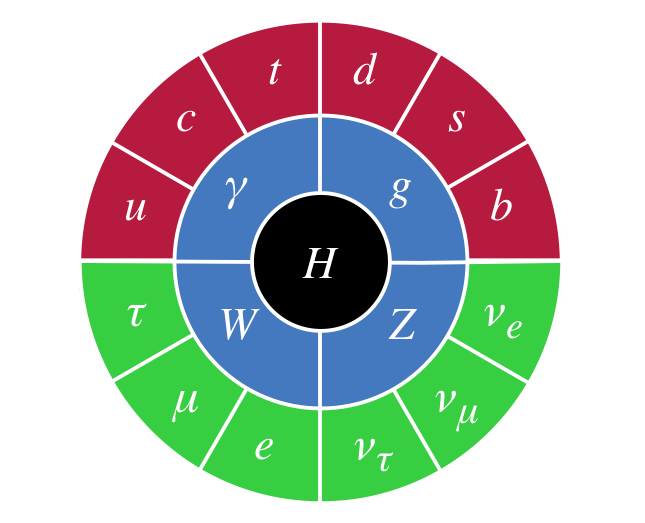
\includegraphics[width=.45\textwidth]{pics/sm_model_particles}
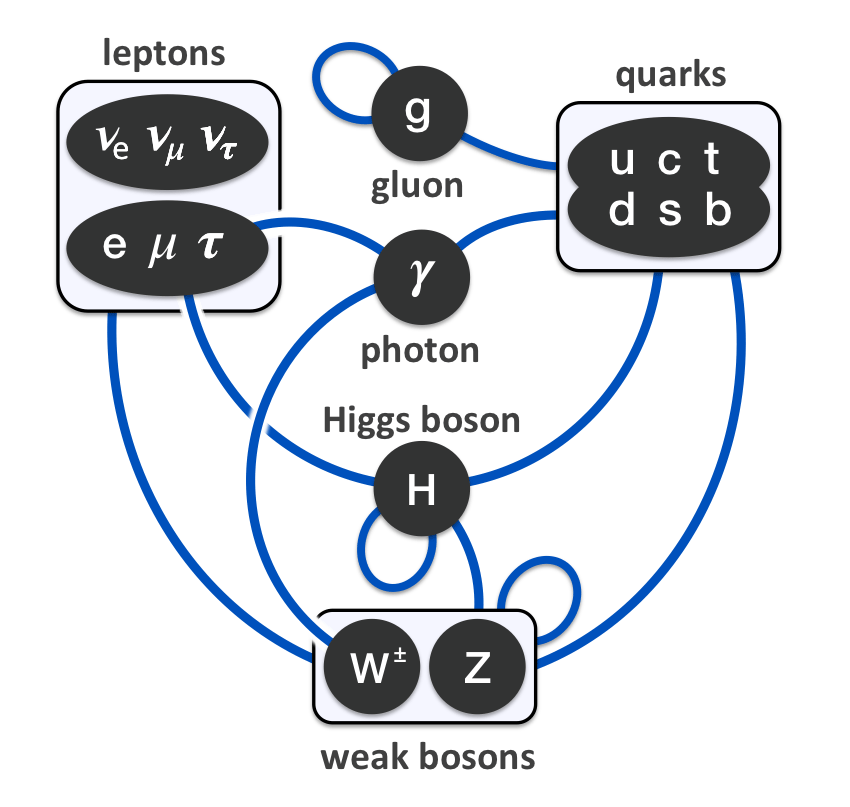
\includegraphics[width=.45\textwidth]{pics/principal_interactions}
\caption{}
\end{center}
\end{figure}

\begin{center}
\begin{table}[]
\begin{center}
\caption{Standard Model particle representations under the symmetry groups $SU(2)$ and $SU(3)$ respectively $n_2$ and $n_3$. Also listed is associated electroweak hypercharge $Y$ as well as the electric charge $Q$ }
\begin{tabular}{cccccccc}
                & $q_L$ & $l_L$  & $u_R$ & $d_R$  & $e_R$ & $\nu_R$ \\
\hline
$n_3$           & 3     & 1      & 3     & 3      & 1     & 1       \\
$n_2$           & 2     & 2      & 1     & 1      & 1     & 1       \\
$Y_{U(1)}$      & 1/6   & $-1/2$ & $2/3$ & $-1/3$ & $-1$  & 0       \\
\hline
\hline
$Q = Y + T_L^3$ & 2/3   & $-1/3$ & 2/3   & $-1/3$ & $-1$  & 0
\end{tabular}
\end{center}
\end{table}
\end{center}

\begin{center}
\begin{table}[]
\begin{center}
\caption{cite-tully-particle: The fundamental fields types contained in the SM Lagrangian}
\begin{tabular}{ccc}
Field & Lagrangian Term & Field Dim. [Mass]\\
\hline
Scalar Field & $(1/2)(\partial_\mu \phi)(\partial^\mu \phi)$ & $[\phi]=M^2$\\
Dirac Field & $\bar \psi M \psi$  & $[\psi]=M^{3/2}$\\
Field Stress Tensor &$-(1/4)F_{\mu\nu}F^{\mu\nu}$ & $[F_{\mu\nu}]=M^2$ \\
Vector Field & $F_{\mu\nu} = \partial_\mu A_\nu - \partial_\nu A_\mu$ & $[A_\mu]=M$\\
\end{tabular}
\label{tab:fields}
\end{center}
\end{table}
\end{center}



\subsection{Re-deriving Maxwell's Laws} 

After, electroweak symmetry breaking we would like to perform a sanity check that we can revive the well estabilished equations of
Maxwell governing electrodynamics. 
Keeping only the terms that contain the field $A_\mu$:
\begin{align*}
\mathcal{L}_{EM} = -\frac{1}{4} F_{\mu\nu} F^{\mu\nu}  - ie \bar{\psi} \gamma^\mu A_\mu \psi \text{ for } F_{\mu\nu} = \partial_\mu A_\nu - \partial_\nu A_\mu 
\end{align*}
where by definition $F_{\mu\nu} = \partial_\mu A_\nu - \partial_\nu A_\mu$. Applying the left side of Euler-Lagrange we find:
\begin{align*}
\partial_\mu \left (\frac{\partial \mathcal L}{\partial(\partial_\mu A_\nu} \right) &=  
-\frac{1}{2}\partial_\mu \left [ \left (\frac{\partial}{\partial(\partial_\mu A_\nu)} F_{\mu\nu} \right) F^{\mu\nu} \right ] 
= - \frac{1}{2} \partial_\mu \left [(1 - \delta^\mu_\nu) F^{\mu\nu} \right ]
= - \frac{1}{2} \partial_\mu F^{\mu\nu}
\end{align*}
The other term is simply $\frac{\partial \mathcal L}{\partial A_\mu} = -ie \bar \psi \gamma^\mu  \psi = J^\mu = (\rho, \vec J)$. Where $\rho$ is charge
density and $\vec J$ is current. This yields our first equation:
\begin{equation}
\partial_\nu F^{\nu\mu} = J^\mu
\end{equation}
recognizing the field tress tensor is antisymmetric we can apply a partial derivative and contract with the indicies of the 4 dimensions anti-symmetric symbol
to obtain:
\begin{equation}
\epsilon_{\theta\rho\mu\nu} \partial{\rho} F_{\mu\nu} = 0 
\end{equation}
Using these two laws and suggestively defining $E^i = F^{0i}$ and $\epsilon^{ijk}B^k = F^{jk}$  simple substitution 

Don't forget that the assumptions to get here were simply the existence of energy terms for the field stress tensor 
and the fermonic field $\psi$ (here the electron) and geometric arguments about the continutity in the derivative 
under the $U(1)$ gauge symmetry in the Lagrangian. Everything we understood about about electromagnetism naturally 
arises (including the gauge freedom of the field $\vec A$). Thats just awesome. 





\section{Beyond the Standard Model}

\subsection{Problems with the Standard Model}

\subsection{Supersymmetry}

\subsection{Electroweak Symmetry Breaking in Supersymmetric Theories}

\section{Origins of Long-lived Signatures}

\subsection{Standard Model Particles with Long Lifetimes}

The standard model already includes a variety of particles that can generate
 displaced vertices (Table \ref{tab:mesons} Table \ref{tab:baryons}). 
For example, $B^0 \rightarrow J/\psi K^{*0}$ with $K^{*0} \rightarrow K^+\pi^-$ 
generates a 4 track vertex. Such a vertex is commonly utilized 
in b-tagging. Of particular interest to single displaced jet identification outside of the b-tagging regime are charge neutral SM particles
decaying to charged particles with a few centimeter lifetime: $\Lambda^0$, $K_S^0$. Such particles would have no track
leading to the primary vertex and vertices far outside the b lifetime. The most relevant of processes being:

\begin{enumerate}
\item $K_s^0 \rightarrow \pi^+\pi^-$ 69\% of all $K_s^0$ decays 
\item $\Lambda^0 \rightarrow p \pi^-$ 64\% of all $\Lambda^0$ decays 
\end{enumerate}

Jets containing prompt and non-prompt $K_s$ and $\Lambda^0$ will contain tracks with large impact parameters, 
and large impact parameter significance. When a vertex is fit to the matched tracks we expect small track multiplicity relative 
to the GeV to TeV   long-lived particles this identification targets. It is important to separate this contribution from
the detector effects like nuclear interactions.


\begin{table}
\begin{center}
\begin{tabular}{cccccc}
\hline
\textbf{Name}  & \textbf{Content}                                    & \textbf{Particle}    & \textbf{mass} (MeV) & $\tau_{0}$ (sec)  & c$\tau$ (cm)         \\
\hline 
Pion & $u\bar{d}$                                  & $\pi^{\pm}$ & 139        & $2.6 \times 10^{-8}$       & $7.8 \times 10^{2}$  \\
\hline 
Kaon  & $u\bar{s}$                                 & $K^{\pm}$   & 497        & $     1.23 \times 10^{-8}$ & $3.7 \times 10^2$    \\
K Short  & $\frac{1}{\sqrt{2}}(d\bar{s} - s \bar{d})$ & $K^0_{s}$   & 497        & $0.896 \times 10^{-10}$    & 2.68                 \\
K Long  & $\frac{1}{\sqrt{2}}(d\bar{s} + s \bar{d})$ & $K^0_L$     & 497        & $5.1\times 10^{-8}$        & $1.5 \times 10^3$    \\
\hline
D & $c\bar{d}$                                 & $D^{\pm}$   & 1869       & $1 \times 10^{-12}$        & $3.0 \times 10^{-2}$ \\
\hline
B meson  & $u \bar{b}$                                & $B^{\pm}$   & 5279       & $1.6 \times 10^{-12}$      & $4.8 \times 10^{-2}$ \\
strange B  & $s\bar{b}$                                 & $B^{0}_s$   & 5366       & $1.5 \times 10^{-12}$      & $4.5 \times 10^{-2}$ \\
charmed B  & $c\bar{b}$                                 & $B^{0}_c$   & 6275       & $4.5\times 10^{-13}$       & $1.4 \times 10^{-2}$ \\
\end{tabular}
\end{center}
\caption{Mesons with Lifetimes greater than $10^{-2}$ cm} 
\label{tab:mesons}
\end{table}


\begin{table}
\begin{center}
\begin{tabular}{cccccc}
\textbf{Name}          & \textbf{Content} & \textbf{Particle}      & \textbf{mass} [MeV] &  $\tau_{0}$ [s] & $c\tau_{0}$ [cm] \\
\hline 
Lambda        & $uds$   & $\Lambda^0$   & 1115       & $2.6 \times 10^{-10}$    & 7.8                  \\
bottom Lambda & $udb$   & $\Lambda^0_b$ & 5620       & $1.4 \times 10^{-12}$    & $4.2 \times 10^{-2}$ \\
\hline
Sigma plus    & $uus$   & $\Sigma^{+}$  & 1189       & $8 \times 10^{-11}$      & 2.4                  \\
Sigma minus   & $dds$   & $\Sigma^{-}$  & 1197       & $1.4\times 10^{-10}$     & 4.2                  \\
\hline 
Xi zero       & $uss$   & $\Xi^0$       & 1314       & $4 \times 10^{-13}$      & $1.2 \times 10^{-2}$ \\
Xi minus      & $dss$   & $\Xi^-$       & 1321       & $1.6 \times 10^{-10}$    & 4.8                  \\
charmed Xi +  & $usc$   & $\Xi^{+}_c$   & 2467       & $4.42 \times 10^{-13}$   & $1.3 \times 10^{-2}$ \\
charmed Xi    & $dsc$   & $\Xi^0_c$     & 2471       & $1.12 \times 10^{-13}$   & $3.3 \times 10^{-2}$ \\
bottom Xi     & $dsb$   & $\Xi^-_b$     & 5792       & $1.56 \times 10^{-12}$   & $4.7 \times 10^{-2}$ \\
\hline
bottom Omega  & $ssb$   & $\Omega_b^-$  & 6054       & $1.13 \times 10^{-12}$   & $3.3 \times 10^{-2}$ \\
Omega minus   & $sss$   & $\Omega^-$    & 1672       & $8 \times 10^{-11}$      & 2.4                  \\
\end{tabular}
\end{center}
\caption{Baryons with Lifetimes greater than $10^{-2}$ cm} 
\label{tab:baryons}
\end{table}


Particles of a characteristic lifetime $\tau$ decay with a falling exponential. For reference, 
a table describing the percent of decays that will occur at various distances is shown in Table
 \ref{tab:lifetime}. Even lifetimes 10 and 100 times the size of the tracker, we would still expect
~10\% and 1\% respectively to occur within the tracker. For particles  of lifetime $\lambda$ we
expect 0.6\% to decay beyond $5\lambda$. 


\begin{table}
\begin{center}
\begin{tabular}{ccc}
Distance ($\lambda$) &  Probability of Decay  \\
\hline
0.01               & 1\%                        \\
0.1                & 9.5\%                      \\              
0.25               & 22\%                       \\            
0.5                & 39\%                       \\          
0.75               & 52\%                       \\        
1                  & 63\%                       \\      
1.5                & 77\%                       \\    
2                  & 86\%                       \\  
3                  & 95\%                       \\
5                  & 99.3\%                     \\
\end{tabular}
\end{center}
\caption{ A reference table for the cumulative probability for a particle of lifetime $\lambda$ to have decayed after a given
distance. Distance is in multiples of lambda.}
\label{tab:lifetime}
\end{table}


\subsection{Split-Susy and Naturalness at the LHC}

The expectation of discovering supersymmetry (SUSY) at the TeV scale has been largely motivated
 by arguments based on naturalness. 
Since the mass of the Standard Model Higgs boson is sensitive to the high energy scale where SUSY
 is broken ($m_{SUSY}$), its mass, of order the electroweak scale, $(m_h \approx m_{EW} \ll m_{SUSY})$
 would need to be tuned to order $m_{EW}^2/m_{SUSY}^2$. 
To avoid fine-tuning, we would like  $m_h^2 \approx m_{SUSY}^2 \implies m_{SUSY} \leq$ 1 TeV. 
More specifically, knowing $m_H \approx 125$ GeV we expect light SUSY partners (in particular, light stops)
 near $< 1$ TeV to stabilize the quadratic divergences of 1 loop corrections to the Higgs mass
 [citation:$light_stops$]. 
Unfortunately these scalar partners have yet to be discovered.

It is important to note that the stability of the Higgs boson mass is not the only
 fine-tuning problem in particle physics. 
When the same argument is made for the cosmological constant we arrive at $\Lambda \geq m_{SUSY}^4$, 
where experimentally $\Lambda = 10^{-59}$ TeV$^4$.   
If we use the same SUSY scale as we did for the Higgs mass,
 $m_{SUSY} = 1$ TeV we have a new fine tuning problem of $10^{60}$.

As addressed by Arkani-Hamed and Dimopoulos [citation:$nima_lhc$], many theoretical approaches  have been
 motivated by a natural explanation for the Higgs mass while separately seeking an  explanation
 of the cosmological constant through some other mechanism.
Arkani-Hamed and Dimopoulos propose a reconsideration of naturalness, entertaining the idea that 
fine tuning could have a role to play in beyond the Standard Model physics.
Conceivably, both $\Lambda$ and $m_h$ fine tuning could be resolved by the same mechanism.  
This un-natural model was  further investigated by Giudice and Romanino [citation:$split_susy$]
and dubbed ``split supersymmetry". 

Split SUSY assumes a much higher SUSY scale $m_{SUSY}^2 \gg 1$ TeV where all scalars (excluding the Higgs) 
become very heavy $O(m_{SUSY})$ and the lightest sparticles (Higgsinos and gluinos) are kept at the TeV scale by requiring the lightest neutralino to be a good dark matter candidate. 

Because the scalars are so much heavier, the decay of gluinos through squarks is suppressed.
The characteristic signature of split supersymmetry is thus long-lived gluinos; such processes 
with long lifetimes are rare in the SM.
